\chapter{Chapter 4: Ranking Algorithms}

\section{Task}
Typically, results returned from search engines are ranked in some way so as to return the more relevant search results first.
The general idea behind this is that for a given website, a score is calculated for each word to indicate the importance of that word on the site.
Then, for intersected searches (that is, searches where all words are required to be present on the webpage for it to be a match) the score is a summation of the scores for each individual word in the search,
and for unioned searches (that is, searches where as long as either part of the union is present on the website it is a match), the score is taken as the maximum of the score for each part of the union search.
For this task, the following ranking algorithms were introduced:

\begin{itemize}

\item Term frequency

\item Term frequency - inverse document frequency

\item Okapi BM25

which are different implementations of the same aforementioned general idea: assigning a score to a search term based on some metric of relevance.

\end{itemize}

\section{Basic Approach}
Research was conducted into the implementations of each of the ranking algorithms.

\begin{itemize}

\item Term frequency
The term frequency (TF) is simply this: given a word and a document (which in this case, is a webpage), how many times does a word appears on the website.
However there are various permutations on this basic formula.
The TF formula settled on in the end was

\begin{equation*}
    term frequency = \frac{number of times the word appears on the website}{number of words on the website}
\end{equation*}

to normalise the score a bit, as a word appearing 10 times on a website 50 words long has a different significance to a word appearing 10 times on a website 500 words long.

\item Term frequency - inverse document frequency
Before the term frequency - inverse document frequency (TFIDF) algorithm can be discussed, the idea behind 'inverse document frequency' must be explained.
The idea behind the inverse document frequency is that while the number of times a word appears on a webpage is a good indication of how important that
word is to that webpage, there are many common words such as 'the', 'and', 'this' etc that will inevitably appear multiple times on a website and will
therefore skew the score of any kind of score based on term frequency.
The inverse document frequency formula is designed to take this into account and is calculated as follows

\begin{equation*}
    inverse document frequency = log_{10}(\frac{number of websites in the search engine index}{number of websites containing the word})
\end{equation*}

Taking the log of this ratio means that the more times a word appears on a website in the database, the closer the IDF gets to 0, and a word that appears on every website
in the database is awarded an IDF value of 0.
That is, common words that are likely to appears on multiple (if not all) websites will have no impact on the ranking score
\\
With that in mind, the meaning behind the TFIDF ranking algorithm becomes clear.
The TFIDF score is calculated as follows:

\begin{equation*}
    TFIDF = TF * IDF
\end{equation*}

The TF score judges the relevance of the word to the website, and the IDF is a weighting to adjust for common words.
Very common words are awarded a TFIDF score of 0 and therefore give no impact in intersected searches.

\item Okapi BM25
The Okapi BM25 algorithm is a more sophisticated type of TFIDF ranking algorithm.
It's a summation over all words that make up the search term, making use of the TF calculation as well as the IDF calculation, with optimisation variables too.
The version of the formula used in this project is:

\begin{equation*}
    okapi BM 25 score = \sum_{i=1}^n IDF(w_i) \cdot \frac{TF(w_i)\cdot (k_1 + 1)}{TF(w_i) + k_1\cdot(1 - b + b\cdot \frac{number of words on the website}{average number of words on a webpage})}
\end{equation*}

with the optimisation variables set as $k_1 = 1.2$ and $b = 0.75$ since no advanced optimisation was considered.
\end{itemize}

It was also decided that the various permutations of Score classes created would be solely responsible for the calculations.
Any required logic was to be handled by the QueryHelper class.

\section{Technical Description}
As per the task description, a generalised {\tt Score} interface was created with only one method: {\tt getScore} which performs the score calculation for the given word with the given website, taking the following parameters:

\begin{itemize}
    \item @param word a word from the search query
    \item @param site the website being scored against the search string
    \item @param index the index of websites
\end{itemize}

and each of the below classes implement this interface.

\begin{figure}[t]
    \centering
    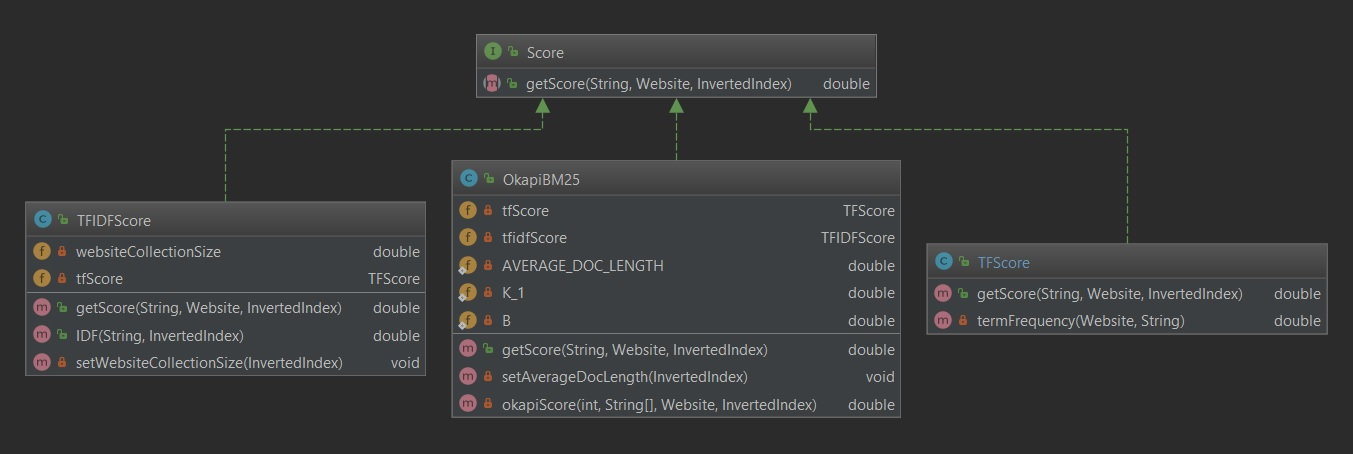
\includegraphics[width=\textwidth]{figures/diagram-score}
    \caption{UML Diagram for the Software Architecture of Score data structures.}
    \label{fig:score:uml}
\end{figure}

\subsection{IFScore class}
The {\tt TFScore} class was the simplest of the three classes to implement, as shown in Figure \ref{fig:score:uml}.
Due to the version of the term frequency formula used in this project, there is a helper method to supplement the required {\tt getScore} method, leaving the {\tt getScore} method to only handle the division.
Due to the changes made to the {\tt FileHelper} class - namely, that no website that lacks a title or words can be created - it's not possible
for there to be a divide by zero error, so no steps were made in this method to account for it.

\subsection{TFIDFScore class}
As the TFIDF makes use of the TF calculation, the {\tt TFIDFScore} class was given a field of type {\tt TFScore} with which to call methods on as needed, rather than creating a new object each time it was required.
Again, helper methods were added to deal with the different aspects of the calculation i.e. the IDF and the number of websites in the search engine index.
The number of websites in the index was built from the index {\tt Map<String, Website>} as below,

\begin{lstlisting}[language=Java]
    private void setWebsiteCollectionSize(InvertedIndex index) {
        Set<Website> siteCollection = new HashSet<>();
        Set<String> words = index.getIndexMap().keySet();
            for(String word : words) {
                List<Website> sites = index.getIndexMap().get(word);
                siteCollection.addAll(sites);
            }
        this.websiteCollectionSize = siteCollection.size();
    }
\end{lstlisting}

making use of the fact that a HashSet allows no duplicates in order to calculate the number of distinct websites in the index.
Again, the {\tt getScore method} only handles the multiplication

\subsection{OkapiBM25 class}
Again, as the Okapi BM25 algorithm makes use of both the TF calculation and the TFIDF calculation, these objects were stored as fields in the {\tt OkapiBM25Score} class as before.
The optimisation constants and the average document length set as static fields.
Two helper methods were added: {\tt setAverageDocLength} and {\tt okapiScore}. {\tt setAverageDocLength} calculates the mean number of words per website based on the websites in the index, and {\tt okapiScore} is a recursive method to perform the summation of all the individual scores of all the words in the search query to return to the {\tt getScore} method.

\begin{lstlisting}[language=Java]
    private double okapiScore(int count, String[] words, Website site, InvertedIndex index) {
        int docLength = site.getWords().size();
        if(count != 0) {
            double IDF = this.tfidfScore.IDF(words[count], index);
            double termFrequency = this.tfScore.getScore(words[count], site, index);
            double score = IDF*((termFrequency*(K_1 + 1))/(termFrequency + K_1*(1 - B + B*(docLength/AVERAGE_DOC_LENGTH))));
            return score + okapiScore(count-1, words, site, index);
        } else {
            double IDF = this.tfidfScore.IDF(words[0], index);
            double termFrequency = this.tfScore.getScore(words[0], site, index);
            return IDF*((termFrequency*(K_1 + 1))/(termFrequency + K_1*(1 - B + B*(docLength/AVERAGE_DOC_LENGTH))));
        }
    }
\end{lstlisting}

\section{Testing considerations}
The correctness of the score calculations were verified using unit tests, which can be found in the ScoreTest.java file.
The set up comprised of building a small index of websites, which allowed for the score values of various words on various
websites to be calculated manually and compared to the results of the {\tt getScore} method.
Each test covered one class, and the individual tests were determined using the standard white-box coverage considerations.
For the tests on the {\tt TFIDFScore} class, a comparison was also included to confirm that a word occurring once on more than one site will have a lower score than a word occurring once on just one site.
For the tests on the {\tt OkapiBM25Score} class, single word and multi word query tests were constructed.

\section{Reflection}
